% !TEX root = supplementary_figures.tex
\documentclass[12pt]{article}

\usepackage[margin=0.75in]{geometry}
\usepackage{fontspec}
\IfFontExistsTF{Times New Roman}{\setmainfont{Times New Roman}}{\setmainfont{TeX Gyre Termes}}
\usepackage{float}
\usepackage{caption}
\usepackage{setspace}
\usepackage{xcolor}
\usepackage{siunitx}
\usepackage{pgfplots}
\usepackage{pgfplotstable}
\usepgfplotslibrary{groupplots}
\usepackage[hidelinks]{hyperref}

\setstretch{1.0}
\setcounter{secnumdepth}{0}
\captionsetup{font=small, labelfont=bf}
\renewcommand{\figurename}{Supplementary Figure}
\renewcommand{\thefigure}{S\arabic{figure}}
\sisetup{round-mode=places, round-precision=4}
\pgfplotsset{compat=1.18}
\pgfplotstableset{col sep=comma}

\newcommand{\DataDir}{../outputs/latex_data}
\definecolor{LogRegColor}{HTML}{E74C3C}
\definecolor{RFColor}{HTML}{2980B9}
\definecolor{HGBColor}{HTML}{27AE60}
\definecolor{MLPColor}{HTML}{8E44AD}
\definecolor{EnsColor}{HTML}{D35400}
\definecolor{UCIRed}{HTML}{C0392B}
\definecolor{NHBlue}{HTML}{2471A3}
\definecolor{TWGreen}{HTML}{1E8449}

\pgfplotsset{
  ckdaxis/.style={
    width=\linewidth,
    height=0.48\linewidth,
    grid=major,
    grid style={draw=gray!20},
    tick align=inside,
    tick pos=left,
    tick style={black},
    tick label style={font=\small},
    label style={font=\small},
    title style={font=\bfseries\small},
    legend style={font=\scriptsize, draw=none, fill=none, cells={anchor=west}},
    unbounded coords=jump
  }
}

\newcommand{\PlotFiveModelCurves}[1]{
  \addplot+[mark=o, thick, color=LogRegColor] table[x=train_size,y=LogReg_test] {#1};
  \addlegendentry{Logistic}
  \addplot+[mark=square*, thick, color=RFColor] table[x=train_size,y=RF_test] {#1};
  \addlegendentry{Random forest}
  \addplot+[mark=triangle*, thick, color=HGBColor] table[x=train_size,y=HGB_test] {#1};
  \addlegendentry{Gradient boosting}
  \addplot+[mark=diamond*, thick, color=MLPColor] table[x=train_size,y=MLP_test] {#1};
  \addlegendentry{MLP}
  \addplot+[mark=*, thick, color=EnsColor] table[x=train_size,y=Ensemble_test] {#1};
  \addlegendentry{Ensemble}
}

\newcommand{\PlotFiveModelCurvesNoLegend}[1]{
  \addplot+[mark=o, thick, color=LogRegColor, forget plot] table[x=train_size,y=LogReg_test] {#1};
  \addplot+[mark=square*, thick, color=RFColor, forget plot] table[x=train_size,y=RF_test] {#1};
  \addplot+[mark=triangle*, thick, color=HGBColor, forget plot] table[x=train_size,y=HGB_test] {#1};
  \addplot+[mark=diamond*, thick, color=MLPColor, forget plot] table[x=train_size,y=MLP_test] {#1};
  \addplot+[mark=*, thick, color=EnsColor, forget plot] table[x=train_size,y=Ensemble_test] {#1};
}

\title{\textbf{Supplementary Information: Figures}\\
\large When Perfect Is Wrong: Exposing the AUC $\approx$ 1.0 Illusion in Chronic Kidney Disease Machine Learning Benchmarks}
\author{}
\date{}

\begin{document}
\maketitle

\noindent This supplementary document contains the figures referenced by the online copy of the manuscript. Figures are reproduced from the LaTeX-native manuscript render using the regenerated CSV outputs.

\begin{figure}[H]
\centering
\begin{tikzpicture}
\begin{axis}[
  ckdaxis,
  ybar,
  bar width=5pt,
  ymin=0.82,
  ymax=1.02,
  symbolic x coords={LogReg,RF,HGB,MLP,Ensemble},
  xtick=data,
  xticklabel style={rotate=25,anchor=east},
  ylabel={AUC-ROC},
  title={Model performance by dataset},
  legend style={at={(0.5,-0.20)}, anchor=north, legend columns=3, font=\scriptsize, draw=none, fill=none}
]
\addplot+[fill=UCIRed, draw=UCIRed] table[x=model,y=UCI] {\DataDir/fig1_model_comparison_wide.csv};
\addlegendentry{UCI}
\addplot+[fill=NHBlue, draw=NHBlue] table[x=model,y=NHANES] {\DataDir/fig1_model_comparison_wide.csv};
\addlegendentry{NHANES}
\addplot+[fill=TWGreen, draw=TWGreen] table[x=model,y=Tawam] {\DataDir/fig1_model_comparison_wide.csv};
\addlegendentry{Tawam}
\end{axis}
\end{tikzpicture}
\caption{UCI is saturated across model families, NHANES with all features is also near-ceiling because of label-feature overlap, and Tawam remains lower and more discriminating among algorithms. The y-axis is intentionally truncated at 0.82 to make small AUC differences visible.}
\end{figure}
\clearpage

\begin{figure}[H]
\centering
\begin{tikzpicture}
\begin{axis}[
  ckdaxis,
  xlabel={UCI training size},
  ylabel={Test AUC-ROC},
  ymin=0.45,
  ymax=1.02,
  xtick={10,20,40,50,75,100,150,200,300},
  title={UCI learning curves},
  legend style={at={(0.5,-0.21)}, anchor=north, legend columns=5, font=\scriptsize, draw=none, fill=none}
]
\PlotFiveModelCurves{\DataDir/fig2_uci_learning_curves_wide.csv}
\end{axis}
\end{tikzpicture}
\caption{UCI performance reaches near-perfect AUC with small stratified subsamples, supporting the ceiling-effect interpretation.}
\end{figure}
\clearpage

\begin{figure}[H]
\centering
\begin{tikzpicture}
\begin{axis}[
  ckdaxis,
  xmode=log,
  xlabel={NHANES training size},
  ylabel={Test AUC-ROC},
  ymin=0.55,
  ymax=1.02,
  title={NHANES learning curves, all features},
  legend style={at={(0.5,-0.21)}, anchor=north, legend columns=5, font=\scriptsize, draw=none, fill=none}
]
\PlotFiveModelCurves{\DataDir/fig3_nhanes_learning_curves_wide.csv}
\end{axis}
\end{tikzpicture}
\caption{With eGFR and ACR included, NHANES approaches a ceiling because the label definition is partly inside the feature set under KDIGO-style eGFR/albuminuria criteria \cite{kdigo2024}.}
\end{figure}
\clearpage

\begin{figure}[H]
\centering
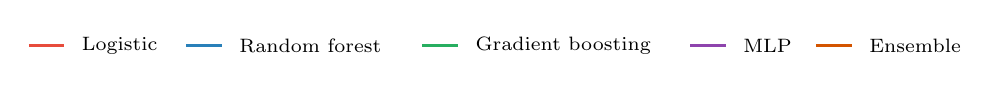
\begin{tikzpicture}
  \draw[thick, color=LogRegColor] (0,0) -- (0.45,0);
  \node[anchor=west, font=\scriptsize] at (0.55,0) {Logistic};
  \draw[thick, color=RFColor] (2.0,0) -- (2.45,0);
  \node[anchor=west, font=\scriptsize] at (2.55,0) {Random forest};
  \draw[thick, color=HGBColor] (5.0,0) -- (5.45,0);
  \node[anchor=west, font=\scriptsize] at (5.55,0) {Gradient boosting};
  \draw[thick, color=MLPColor] (8.4,0) -- (8.85,0);
  \node[anchor=west, font=\scriptsize] at (8.95,0) {MLP};
  \draw[thick, color=EnsColor] (10.0,0) -- (10.45,0);
  \node[anchor=west, font=\scriptsize] at (10.55,0) {Ensemble};
\end{tikzpicture}

\vspace{0.9em}

\begin{tikzpicture}
\begin{groupplot}[
  group style={group size=1 by 3, vertical sep=2.65cm},
  width=0.88\textwidth,
  height=0.22\textwidth,
  grid=major,
  grid style={draw=gray!20},
  xmode=log,
  ymin=0.55,
  ymax=1.02,
  tick align=inside,
  tick pos=left,
  tick label style={font=\small},
  label style={font=\small},
  xlabel style={yshift=-0.25em},
  title style={font=\bfseries\small},
  unbounded coords=jump
]
\nextgroupplot[title={All features}, ylabel={Test AUC}]
\PlotFiveModelCurvesNoLegend{\DataDir/fig9_nhanes_all_wide.csv}
\nextgroupplot[title={No eGFR/ACR}]
\PlotFiveModelCurvesNoLegend{\DataDir/fig9_nhanes_no_egfr_acr_wide.csv}
\nextgroupplot[title={No eGFR/ACR/Cr/BUN}, xlabel={Training size}]
\PlotFiveModelCurvesNoLegend{\DataDir/fig9_nhanes_no_lab_surrogates_wide.csv}
\end{groupplot}
\end{tikzpicture}
\caption{Removing label-defining and closely related laboratory variables exposes a substantially harder NHANES prediction task, especially for logistic regression.}
\end{figure}
\clearpage

\begin{figure}[H]
\centering
\begin{tikzpicture}
\begin{axis}[
  ckdaxis,
  xlabel={Tawam training size},
  ylabel={AUC-ROC},
  ymin=0.45,
  ymax=1.03,
  xtick={20,30,40,50,75,100,125,150,200,368},
  title={Tawam learning curves with train/test gap},
  legend style={at={(0.5,-0.21)}, anchor=north, legend columns=3, font=\scriptsize, draw=none, fill=none}
]
\PlotFiveModelCurves{\DataDir/fig4_tawam_learning_curves_wide.csv}
\addplot+[mark=none, dashed, thick, color=HGBColor] table[x=train_size,y=HGB_train] {\DataDir/fig4_tawam_learning_curves_wide.csv};
\addlegendentry{HGB train}
\end{axis}
\end{tikzpicture}
\caption{Tawam test AUC improves with additional data. The dashed gradient-boosting training curve shows the monitored overfitting gap.}
\end{figure}
\clearpage

\begin{figure}[H]
\centering
\pgfplotstableread[col sep=comma]{\DataDir/fig5_single_feature_auc.csv}\singlefeaturedata
\begin{tikzpicture}
\begin{axis}[
  ckdaxis,
  xbar,
  width=0.88\linewidth,
  height=0.64\linewidth,
  xmin=0.40,
  xmax=1.02,
  xlabel={Single-feature AUC-ROC},
  ytick=data,
  yticklabels from table={\singlefeaturedata}{display_name},
  yticklabel style={font=\scriptsize, text width=3.0cm, align=right},
  title={UCI single-feature discriminability}
]
\addplot+[fill=UCIRed, draw=UCIRed] table[x=auc,y expr=\coordindex] {\singlefeaturedata};
\draw[dashed, thick, gray] (axis cs:0.90,-1) -- (axis cs:0.90,14);
\end{axis}
\end{tikzpicture}
\caption{Several individual UCI features approach or exceed AUC 0.90 on their own.}
\end{figure}
\clearpage

\begin{figure}[H]
\centering
\begin{tikzpicture}
\begin{axis}[
  ckdaxis,
  ybar,
  width=0.96\linewidth,
  bar width=6pt,
  ymin=0.98,
  ymax=1.002,
  symbolic x coords={LogReg,RF,HGB,MLP,Ensemble},
  xtick=data,
  xticklabel style={rotate=25,anchor=east},
  ylabel={AUC-ROC},
  title={UCI top-feature ablation},
  ytick={0.98,0.985,0.99,0.995,1.0},
  yticklabel style={/pgf/number format/fixed,/pgf/number format/precision=3},
  legend style={at={(0.5,-0.22)}, anchor=north, legend columns=2, font=\scriptsize, draw=none, fill=none}
]
\addplot+[fill=UCIRed, draw=UCIRed] table[x=model,y=original_auc] {\DataDir/fig10_ablation.csv};
\addlegendentry{Original}
\addplot+[fill=TWGreen, draw=TWGreen] table[x=model,y=ablated_auc] {\DataDir/fig10_ablation.csv};
\addlegendentry{Top 3 removed}
\end{axis}
\end{tikzpicture}
\caption{Top-feature removal barely lowers UCI performance. The 0.98-truncated y-axis makes the near-ceiling range visible.}
\end{figure}
\clearpage

\begin{figure}[H]
\centering
\begin{tikzpicture}
\begin{axis}[
  ckdaxis,
  ybar,
  bar width=5pt,
  ymin=0,
  ymax=1.03,
  symbolic x coords={LogReg,RF,HGB,MLP,Ensemble},
  xtick=data,
  xticklabel style={rotate=25,anchor=east},
  ylabel={AUC-ROC},
  title={UCI-trained cross-dataset transfer},
  legend style={at={(0.5,-0.20)}, anchor=north, legend columns=3, font=\scriptsize, draw=none, fill=none}
]
\addplot+[fill=UCIRed, draw=UCIRed] table[x=model,y=UCI_self_commonfeats] {\DataDir/fig6_cross_dataset_wide.csv};
\addlegendentry{UCI to UCI}
\addplot+[fill=NHBlue, draw=NHBlue] table[x=model,y=UCI_to_NHANES] {\DataDir/fig6_cross_dataset_wide.csv};
\addlegendentry{UCI to NHANES}
\addplot+[fill=TWGreen, draw=TWGreen] table[x=model,y=UCI_to_Tawam] {\DataDir/fig6_cross_dataset_wide.csv};
\addlegendentry{UCI to Tawam}
\end{axis}
\end{tikzpicture}
\caption{UCI-trained models do not reliably transfer to NHANES or Tawam even when the feature space is restricted to shared clinical variables.}
\end{figure}
\clearpage

\begin{figure}[H]
\centering
\begin{tikzpicture}
\begin{groupplot}[
  group style={group size=2 by 1, horizontal sep=1.3cm},
  width=0.47\textwidth,
  height=0.38\textwidth,
  grid=major,
  grid style={draw=gray!20},
  xmin=0,
  xmax=1,
  ymin=0,
  ymax=1.02,
  xlabel={False positive rate},
  ylabel={True positive rate},
  tick label style={font=\scriptsize},
  label style={font=\scriptsize},
  title style={font=\bfseries\small},
  unbounded coords=jump
]
\nextgroupplot[title={UCI CKD}]
\addplot+[mark=none, thick, color=LogRegColor] table[x=fpr,y=tpr] {\DataDir/fig7_roc_uci_LogReg.csv};
\addplot+[mark=none, thick, color=RFColor] table[x=fpr,y=tpr] {\DataDir/fig7_roc_uci_RF.csv};
\addplot+[mark=none, thick, color=HGBColor] table[x=fpr,y=tpr] {\DataDir/fig7_roc_uci_HGB.csv};
\addplot+[mark=none, thick, color=MLPColor] table[x=fpr,y=tpr] {\DataDir/fig7_roc_uci_MLP.csv};
\addplot+[mark=none, thick, color=EnsColor] table[x=fpr,y=tpr] {\DataDir/fig7_roc_uci_Ensemble.csv};
\addplot+[mark=none, dashed, gray] coordinates {(0,0) (1,1)};
\nextgroupplot[title={Tawam UAE}]
\addplot+[mark=none, thick, color=LogRegColor] table[x=fpr,y=tpr] {\DataDir/fig7_roc_tawam_LogReg.csv};
\addplot+[mark=none, thick, color=RFColor] table[x=fpr,y=tpr] {\DataDir/fig7_roc_tawam_RF.csv};
\addplot+[mark=none, thick, color=HGBColor] table[x=fpr,y=tpr] {\DataDir/fig7_roc_tawam_HGB.csv};
\addplot+[mark=none, thick, color=MLPColor] table[x=fpr,y=tpr] {\DataDir/fig7_roc_tawam_MLP.csv};
\addplot+[mark=none, thick, color=EnsColor] table[x=fpr,y=tpr] {\DataDir/fig7_roc_tawam_Ensemble.csv};
\addplot+[mark=none, dashed, gray] coordinates {(0,0) (1,1)};
\end{groupplot}
\end{tikzpicture}

\vspace{0.5em}
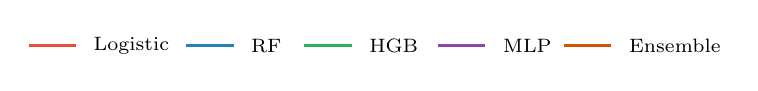
\begin{tikzpicture}
  \draw[thick, color=LogRegColor] (0,0) -- (0.6,0);
  \node[anchor=west, font=\scriptsize] at (0.7,0) {Logistic};
  \draw[thick, color=RFColor] (2.0,0) -- (2.6,0);
  \node[anchor=west, font=\scriptsize] at (2.7,0) {RF};
  \draw[thick, color=HGBColor] (3.5,0) -- (4.1,0);
  \node[anchor=west, font=\scriptsize] at (4.2,0) {HGB};
  \draw[thick, color=MLPColor] (5.2,0) -- (5.8,0);
  \node[anchor=west, font=\scriptsize] at (5.9,0) {MLP};
  \draw[thick, color=EnsColor] (6.8,0) -- (7.4,0);
  \node[anchor=west, font=\scriptsize] at (7.5,0) {Ensemble};
\end{tikzpicture}
\caption{ROC curves collapse near the upper-left corner on UCI, while Tawam preserves more visible separation.}
\end{figure}
\clearpage

\begin{figure}[H]
\centering
\begin{tikzpicture}
\begin{groupplot}[
  group style={group size=1 by 3, vertical sep=1.55cm},
  width=0.88\textwidth,
  height=0.28\textwidth,
  grid=major,
  grid style={draw=gray!20},
  xmode=log,
  ymin=0.55,
  ymax=1.02,
  tick align=inside,
  tick pos=left,
  tick label style={font=\small},
  label style={font=\small},
  title style={font=\bfseries\small},
]
\nextgroupplot[title={All features}, ylabel={HGB AUC}]
\addplot+[only marks, mark=o, color=HGBColor, forget plot] table[x=train_size,y=observed_hgb] {\DataDir/fig8_powerlaw_all.csv};
\addplot+[mark=none, thick, dashed, color=UCIRed, forget plot] table[x=train_size,y=fit_hgb] {\DataDir/fig8_powerlaw_all.csv};
\nextgroupplot[title={No eGFR/ACR}, ylabel={HGB AUC}]
\addplot+[only marks, mark=o, color=HGBColor, forget plot] table[x=train_size,y=observed_hgb] {\DataDir/fig8_powerlaw_no_egfr_acr.csv};
\addplot+[mark=none, thick, dashed, color=UCIRed, forget plot] table[x=train_size,y=fit_hgb] {\DataDir/fig8_powerlaw_no_egfr_acr.csv};
\nextgroupplot[title={No eGFR/ACR/Cr/BUN}, xlabel={Training size}, ylabel={HGB AUC}]
\addplot+[only marks, mark=o, color=HGBColor, forget plot] table[x=train_size,y=observed_hgb] {\DataDir/fig8_powerlaw_no_lab_surrogates.csv};
\addplot+[mark=none, thick, dashed, color=UCIRed, forget plot] table[x=train_size,y=fit_hgb] {\DataDir/fig8_powerlaw_no_lab_surrogates.csv};
\end{groupplot}
\end{tikzpicture}

\vspace{0.5em}
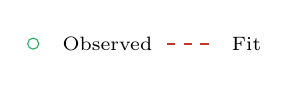
\begin{tikzpicture}
  \draw[only marks, mark=o, color=HGBColor] plot coordinates {(0,0)};
  \node[anchor=west, font=\scriptsize] at (0.25,0) {Observed};
  \draw[thick, dashed, color=UCIRed] (1.7,0) -- (2.3,0);
  \node[anchor=west, font=\scriptsize] at (2.4,0) {Fit};
\end{tikzpicture}
\caption{Power-law fits summarize NHANES learning behavior under the three feature definitions. The ceiling parameter is descriptive and constrained by AUC's upper bound.}
\end{figure}

\begin{thebibliography}{1}
\bibitem{kdigo2024} KDIGO CKD Work Group. KDIGO 2024 clinical practice guideline for the evaluation and management of chronic kidney disease. \emph{Kidney International.} Vol. 105, No. 4S, pg. S117--S314, 2024, DOI: \url{https://doi.org/10.1016/j.kint.2023.10.018}.
\end{thebibliography}

\end{document}
